\section{Introduction}

Automatic image localization continues to grow in importance as a
direct result of the increasing amount of imagery available
via the Internet. Conceptually the task is straightforward; given an
image, identify the location it was captured in the world directly
from image data. Solving this problem is of great value for a wide
variety of fields, with potential applications ranging from the
forensic sciences~\cite{stylianou13jane} to crowd-sourced
environmental monitoring~\cite{zhang2012mining}.

\begin{figure}
  
  \centering

  \begin{subfigure}{.84\linewidth}
    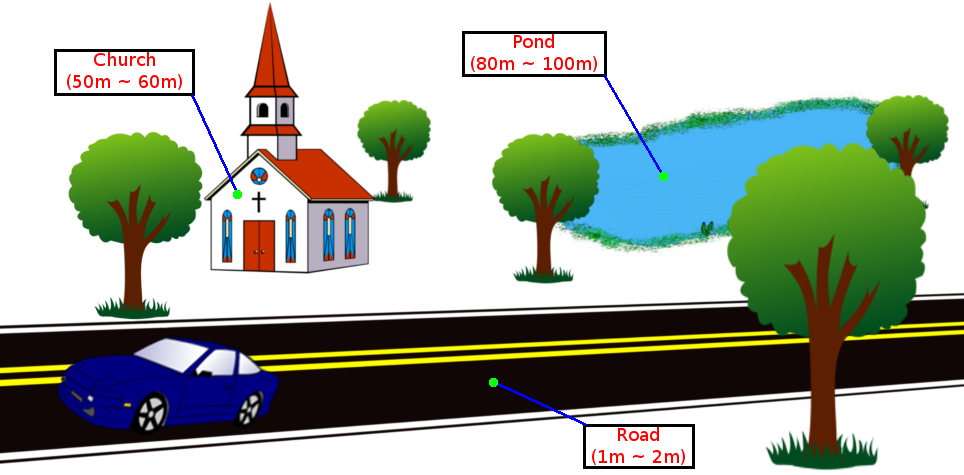
\includegraphics[width=\linewidth]{mcmc/image_frame}
    %\caption{Labeled query image}
  \end{subfigure}
  \begin{subfigure}{.41\linewidth}
    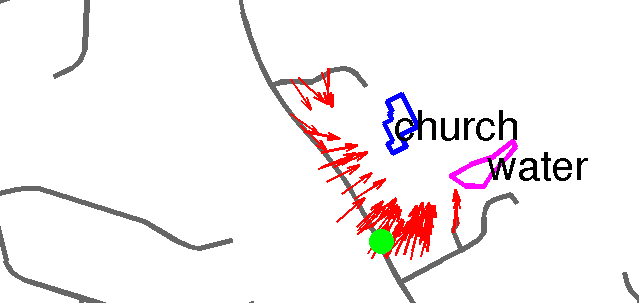
\includegraphics[width=\linewidth]{mcmc/mcmc_direction}
    %\caption{GIS reference data and best sampled cameras (red arrows)}
  \end{subfigure}
  \begin{subfigure}{.41\linewidth}
    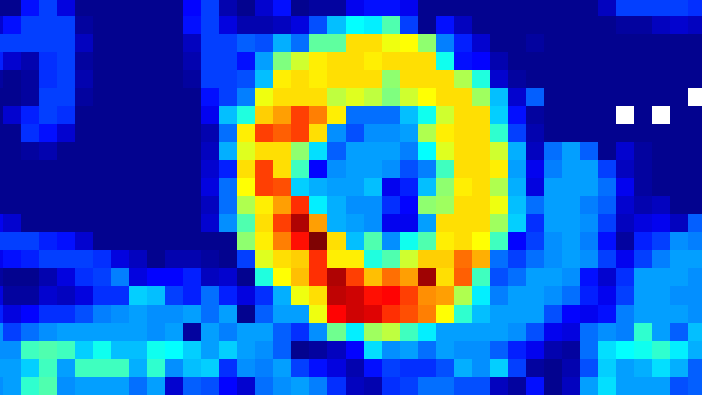
\includegraphics[width=\linewidth]{mcmc/mcmc_score}
    %\caption{Probability distribution over camera location}
  \end{subfigure}

  \caption{We match objects in an image (top) to GIS reference data
  (left) to estimate a probability distribution over locations
(right).  The map (left) also shows the true camera location (green
dot) and the top scoring sampled cameras (red arrows).}

\label{fig:cartoon}

\end{figure}

However, recognizing the geo-location and geo-orientation of an
arbitrary outdoor image is an extremely challenging task.  Many
methods have been proposed; the most common approach is to build a
large database of images with known location and localize a query
image using either local~\cite{li2010location,schindler2008detecting}
or global~\cite{hays2008im2gps,doersch2012what} image features.  This
approach is not applicable when no nearby ground-level imagery exists
in the reference database, such as when the image was not captured
near a popular tourist destination.  Even
when reference imagery is available, the appearance of the objects may
not be visually distinctive, for example a train track or a body of
water. 

Instead of matching visually against a reference image set, we exploit
the large quantities of publicly available geospatial data to build a
geographic database containing geometric information for objects of
interest in the world, such as roads, churches, bodies of water, water
towers and golf courses.  Given a query image, we identify visible
objects of interest in the image and apply the Metropolis-Hastings
MCMC algorithm to randomly sample possible cameras.  We assign a score
to each hypothetical camera and use these samples to approximate the
probability distribution over the camera parameters and extract
candidate locations. \figref{cartoon} gives an brief view of our
approach.

Our key contributions are: 1) a flexible approach to the camera
geo-calibration problem that supports priors over camera parameters
and constraints that relate image annotations, camera geometry, and a
geographic database and 2) an extensive comparison of this approach to
uniform and grid-based sampling on real-world data.

\subsection{Related Work}

\begin{figure}[t]

  \centering

  \frame{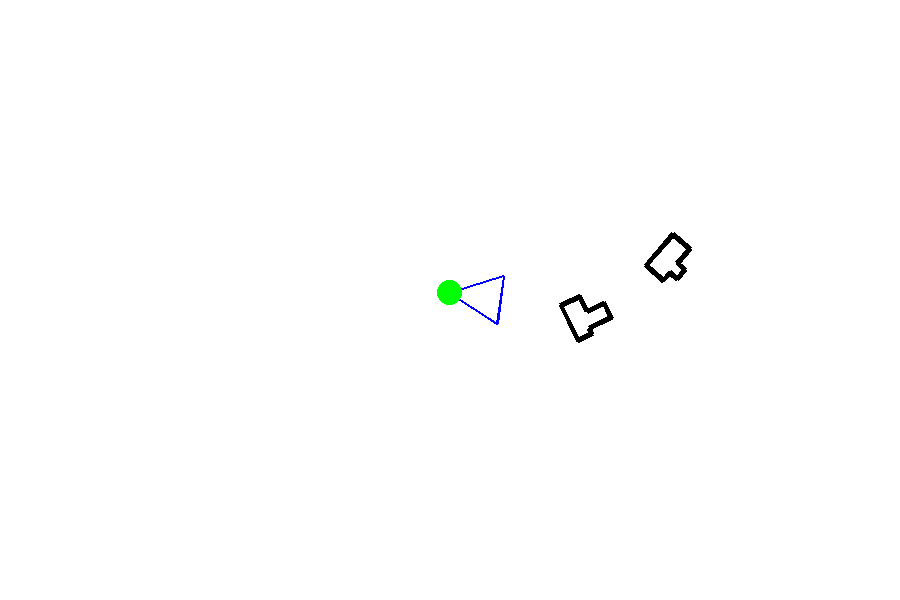
\includegraphics[width=.3\linewidth]{mcmc/diffmodel_map}}
  \hfill
  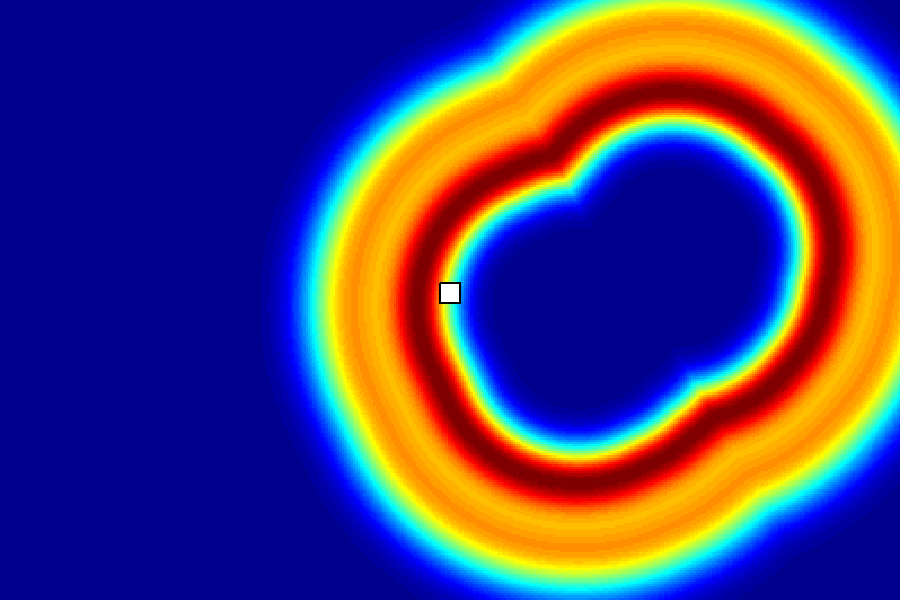
\includegraphics[width=.3\linewidth]{mcmc/distance_scoring}
  \hfill
  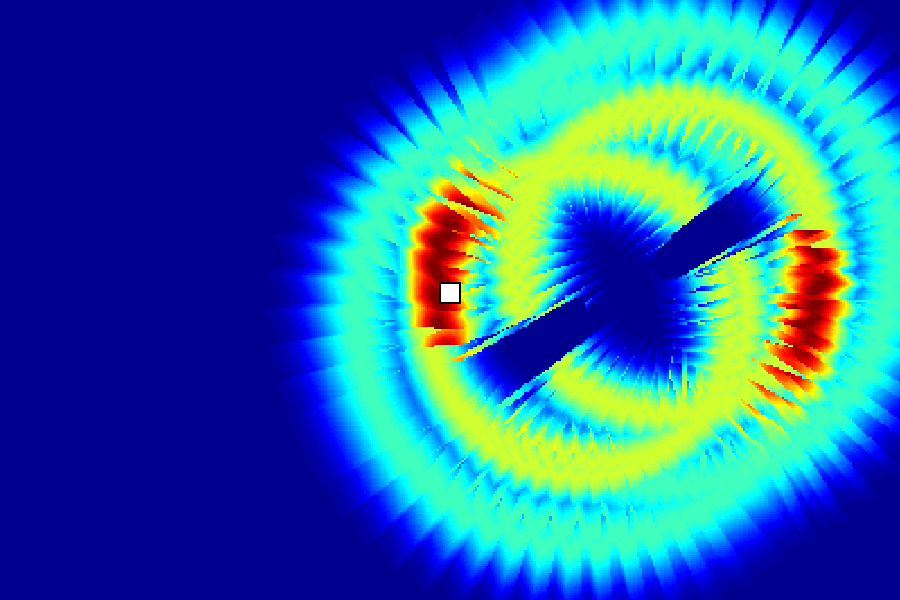
\includegraphics[width=.3\linewidth]{mcmc/fullmodel_scoring}

  \caption{(left) A map showing two houses (black) and a hypothetical
    ground-truth camera frustum. (middle) The PDF (red is high
    probability) over location for a 2D camera model, in which
    constraints are based on distances between the camera and GIS
  objects. (right) The 4D model we propose enables richer constraints,
  which leads to a more accurate PDF.}

  \label{fig:diffmodel}
\end{figure}

Self-localization has been heavily studied in the robotics community. The task is to
estimate the probability density function (PDF) over the robot's state
space (location and orientation). Early methods attempted to estimate
this density by discretizing the state
space~\cite{burgard1996estimating}. These grid-based approaches
suffered from large computational overhead and memory requirements. To
overcome these limitations, probabilistic particle-based methods like
MCMC were
investigated~\cite{dellaert1999using,fox1999monte,gutmann1998experimental,oh2004map}.
The idea is to approximate the probability density using randomly drawn
samples, while maintaining performance even for high dimensional state
spaces.

Extracting location-dependent features from image data has drawn a
great detail of attention from the vision
community~\cite{jacobs07geolocate, jacobs11geolocate,
jacobs08geoorient}. The common trend amongst these methods is that
they take advantage of a large dataset of geo-referenced images. Hays
and Efros~\cite{hays2008im2gps} use a data-driven scene matching
approach to localize a query image using a large dataset of geo-tagged
images.  Doersch et al. extract location-dependent features that
capture the relative appearance differences of large cities.  Lin et
al.~\cite{lin2013cross} localize a ground-level image by learning the
relationship between pairs of ground and aerial images of the same
location. Other techniques focus on urban environments and infer
location using local image
descriptors~\cite{schindler2008detecting,snavely2006photo}. Li et
al.~\cite{li2012worldwide} exploit geo-registered 3D points clouds to
estimate camera pose. Many other cues exist, such as the
skyline~\cite{baatz2012large,ramalingam2009geolocalization}, sky
appearance~\cite{lalonde2010sun,workman2014rainbow}, and
shadows~\cite{junejo2008estimating,wu2010geo}.

Our work attempts to combine these two research directions. We use
publicly available geospatial data to build a large geographic
database containing geometric information for objects in the world,
identify objects of interest in the query image, and use a
probabilistic approach to estimate camera geo-calibration. To our
knowledge, our approach is the first to apply a probabilistic
particle-based MCMC algorithm for single image camera geo-calibration
using a large geographic database. 


\section{Approach}

Given a query image, captured at an unknown location in a known region
of interest (ROI) and annotated with the location of geographic objects
(e.g., buildings and roads), our goal is to estimate the intrinsic and
extrinsic camera parameters.  We base these estimates on a geographic
information system (GIS) database that contains the location and
extent of objects in the ROI.  Assuming a simplified
pinhole camera model
with square pixels and zero skew, the full camera geo-calibration
problem is seven-dimensional: three position parameters, three
orientation parameters, and the field of view. For this work, we
assume that most photos are taken about five feet above the ground
with little tilt or roll and reduce our model to four dimensions:
$\Theta = (Latitude, Longitude, Azimuth, FOV)^\mathsf{T}$. 
%
Adapting to higher or lower dimensional camera models is
straightforward and may be useful depending on the available image
annotations and GIS data.  We find our proposed 4D state space to be
good trade-off between the lack of descriptive power of lower-order
camera models and higher-order camera models that require more
computational time and memory resources. See \figref{diffmodel} for an
% scott review
example that compares our proposed model to a 2D model using only
location.

Since one-to-one matching between image objects and GIS objects is
likely not possible, we instead seek to estimate, $f(\Theta;
\mathbf{C})$, the probability distribution function (PDF) over the
camera parameters, $\Theta$, given a set of constraints, $\mathbf{C}$.
In the following section, we propose a function (an unnormalized
density) that encodes constraints on the geo-calibration.  This score
function, $S(\Theta; \mathbf{C})$, encodes both prior knowledge about
the camera and the geometric relationship between image annotations
and the geographic database.
%
In \secref{mcmc} we show how to estimate $f(\Theta;\mathbf{C})$ by
sampling from this scoring function using an MCMC-based strategy.

\subsection{Scoring Function}
\label{sec:scoring-function}

Proportional to the probability distribution of the camera parameters,
$f(\Theta; \mathbf{C})$, the scoring function, $S(\Theta;
\mathbf{C})$, is defined as a linear combination of multiple constraint
functions:
%
\begin{equation}
  S(\Theta; \mathbf{C}) = \sum_{}{w_i g(c_i, \Theta)} \propto
  f(\Theta; \mathbf{C}),
\end{equation}
%
where $w_i$ is a weight and $g(c_i, \Theta)$ is a constraint function
which is larger if the calibration, $\Theta$, is more consistent with
the image information, $c_i$. 
%
While the scoring function can take any type of constraint functions,
we define a variety of functions in our implementation, including
geometric configuration of multiple weak correspondences, constraints
on geographic location, and priors over the field of view and camera
orientation, to demonstrate the performance of our model. 
%
%While the exact set of constraints
%depends on the image and database contents, we define a variety of
%functions in our implementation, including geometric configuration of
%multiple weak correspondences, constraints on geographic location, and
%priors over the field of view and camera orientation. 
%
We focus on the first constraint specifically, the latter are simple
Gaussian and uniform distributions. 

\begin{figure}
\begin{minipage}[b]{1\linewidth}
  \centering
  \centerline{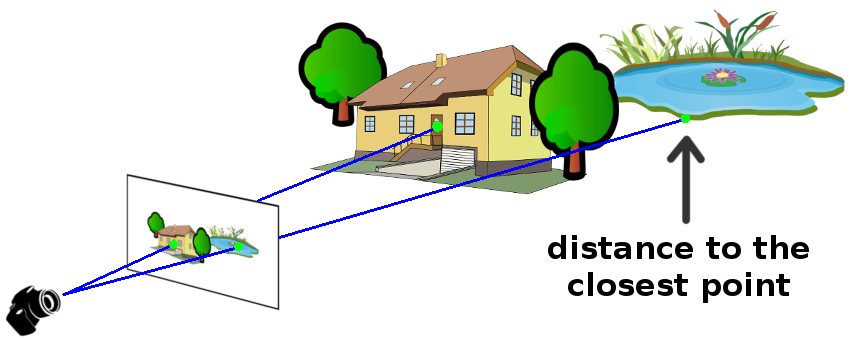
\includegraphics[width=.8\linewidth]{mcmc/scoring_demo}}
\end{minipage}
\caption{Since the exact correspondence between an image pixel and a point
  on a GIS object is unknown, we compute the distance to the closest
  point of the object to compare with the estimated distance.}
\label{fig:scoring-demo}
\end{figure}

% scott review
Given the extent of an object in the image, and an
%
estimated range of distances, $(d_{min},d_{max})$, from the camera to
the object, we propose a constraint function that measures the
geometric consistency between the object in the image and the GIS
database. Given a hypothetical camera, $\Theta$, we compute the
distance, $d$, from the camera, through the object pixel, to the
closest point of the object (see \figref{scoring-demo}), then the
consistency function, $g(c_i, \Theta)$, takes form of a Gaussian
distribution function, with mean $\mu = d - (d_{min} + d_{max})/2$,
and standard deviation $\sigma = d_{max} - d_{min} + o$, where $o$ is
a constant offset ($o=10 m$ for all our experiments) to avoid dividing
by zero. If no object of the correct type intersects the pixel ray,
let $g(c_i, \Theta) = 0$.

\subsection{Monte Carlo Markov Chain}
\label{sec:mcmc}

The MCMC method is an efficient approach for sampling from high
dimensional spaces. Its principal advantage over naive sampling
strategies is that it visits high probability areas more frequently
than the areas of low probability.  We use the Metropolis-Hastings
(MH) algorithm~\cite{chib1995understanding}, a popular member of the
MCMC family.  The algorithm generates a set of possible cameras as
follows: randomly sample a camera and compute its score; randomly
sample (propose) a new nearby camera and compute its score; if the
score of the new camera is higher, replace the old camera with the new
camera, otherwise replace the old probabilistically; repeat this
process many times, recording samples along the way. After a
sufficiently large number of iterations, this process generates a set
of possible cameras that are independent samples from the PDF,
$f(\Theta;\mathbf{C})$, subject to some technical conditions. See
\algref{MH-algorithm} for details of the MH algorithm. We run multiple
chains to mitigate issues with poor initial samples and local maxima.

\begin{algorithm}[t]
  \caption{Metropolis-Hastings Algorithm (MCMC)}
  \begin{algorithmic}[1]
    \REQUIRE $\mathbf{C}$ (constraint set), and $maxIter$
    \STATE Initialize camera parameters, $\Theta_0$
    \STATE $i \gets 0,~~ \mathbb{S} \gets \emptyset,~~s_0 \gets S(\Theta_0;
    \mathbf{C})$
    \WHILE{ $i < maxIter$ }
       \STATE sample new camera parameters: $\Theta_{i+1}$ \label{alg:stp:sampling}
       \STATE scoring: $s_{i+1} \gets S(\Theta_{i+1}; \mathbf{C})$
       \STATE $\mathbb{S} \gets \mathbb{S} \cup \langle\Theta_{i+1}, s_{i+1}\rangle$
       \IF{ $s_{i+1} < s_i$ }
       \STATE $s_{i+1} \gets s_i,~~\Theta_{i+1} \gets \Theta_i$ with 
       %\newline
       prob. $\frac{s_i - s_{i+1}}{s_i}$
       \ENDIF
       \STATE $i \gets i + 1$
    \ENDWHILE
    \STATE \Return $\mathbb{S}$
  \end{algorithmic}
  \label{alg:MH-algorithm}
\end{algorithm}

Aside from the scoring function, $S(\Theta;\mathbf{C})$, the proposal
distribution, $p(\Theta)$, which specifies how new cameras are
sampled from a current camera
(\algref{MH-algorithm}.\textcolor{red}{$4$}), is the most important
choice when using an MCMC approach. We use the joint distribution of
independent Gaussian random variables:
%
\begin{displaymath}
  p(\Theta_{i+1} \given \Theta_i) = \prod_{j =
  1}^{N_{dim}}{\frac{1}{\sigma_j}\phi\left(\frac{\Theta_{i+1,j} -
\Theta_{i,j}}{\sigma_j}\right)},
\end{displaymath}
where $\sigma_j$ denotes the sampling step size on the $j$-th
dimension, and $\phi(x)$ denotes the PDF of the standard normal
distribution. As with all MH-based algorithms, the sampling
performance is sensitive to the choice of step size. If the step size
is too large, the algorithm converges slowly; if too small, the Markov
chain may be trapped in a local maximum. 

\section{Evaluation}
\label{sec:evaluation}

We compare our approach with two baseline methods, grid sampling and
uniform random sampling, on real-world GIS data. The quantitative and
qualitative results demonstrate the value of the proposed MH-based
approach.

\begin{figure}
  \centering
  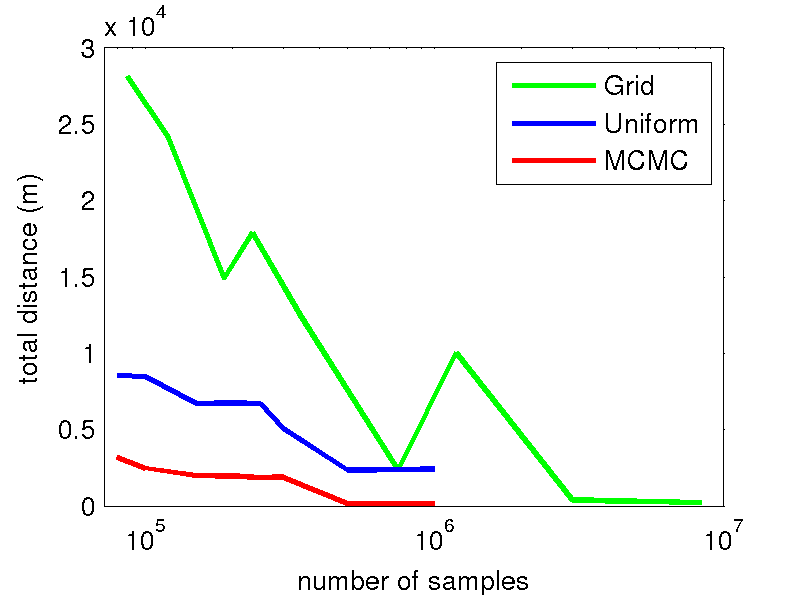
\includegraphics[width=.49\linewidth]{mcmc/total_distance}
  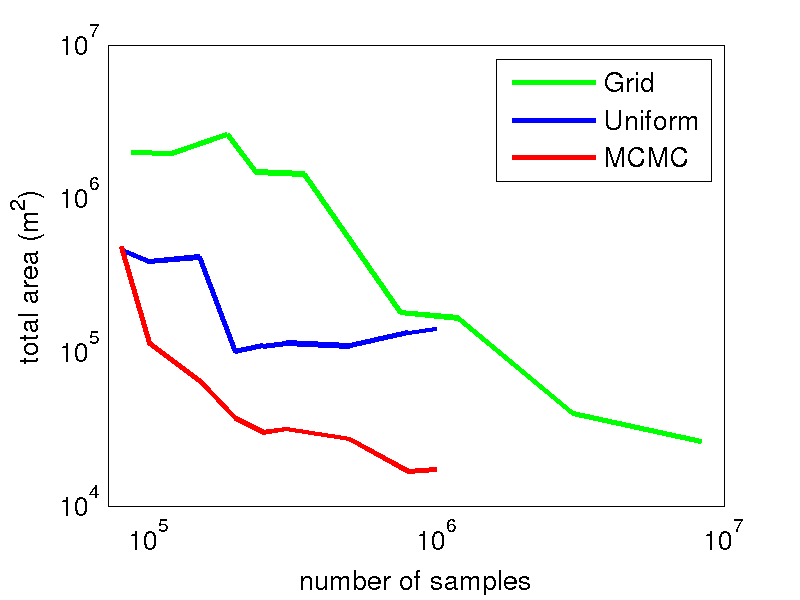
\includegraphics[width=.49\linewidth]{mcmc/total_area}
  \caption{Performance comparison among methods. (left) Total
    distance. (right) Total area. For the grid method the finest
    sampling over spatial dimensions is 30m.}
  \label{fig:comparison}
\end{figure}

\subsection{Methods}

\textbf{Dataset:} 
We build a reference geographic database from
OpenStreetMap\footnote{\url{http://www.openstreetmap.org}} data, which
contains the location and extent of many types of objects around the
world. We only include roads, water, churches, residential buildings,
and commercial buildings. For each query, we focus on a different
$5km\times5 km$ ROI, in Kentucky, USA, each containing approximately
$900$ objects.

\noindent
\textbf{Metrics:}
We propose two evaluation metrics that simulate the process of
manually verifying the camera location. For both, we generate a
candidate list by sorting samples by their scores, then scan from the
top until the ground-truth location is found.
Given a set of samples from the state space and
their corresponding scores, we greedily select the top-$N$ candidates
in terms of score, subject to the constraint that each of them is at
least 200 meters away from the others spatially. Then, if the $k$-th
candidate is the first candidate that is $d$ ($d < 100$) meters away
from the ground truth, we define its {\em total distance} to the ground
truth as follows: $T_d = 200(k-1) + d$.
Intuitively, this metric enforces the diversity of candidate
locations. The first term penalizes the ranking
of the ground-truth candidate. The distance, $d$, distinguishes the
accuracy of predictions in the case that two ground-truth candidate
locations have the same ranking. By definition, a lower total distance
to find the ground-truth candidate is better.
The definition of the {\em total area}, $T_a$, is similar: we center a
$l \times l$ patch around each candidate and compute the union of the
areas from the top candidate patch to the patch that covers the
ground-truth location. We set $l$ to be $50m$ initially, if no patch
covers the ground truth, we double the size of $l$ and redo the
computation until the ground-truth location is covered.

\noindent
\textbf{Implementation Details:}
We use the following fixed set of parameters, which we selected
empirically, for all experiments. The ranges from which azimuth and
FOV are sampled are $[0, 2\pi]$ and $[\pi/3, 2\pi/3]$
respectively. For the grid method, 50 angles are evenly sampled for
azimuth, and 6 for the field of view. Thus at each geographic
location, a total of $300$ scoring samples are generated. For MCMC, 200
chains are independently processed in parallel. The step size is 100m
for location, $\pi/20$ for azimuth, and $\pi/30$ for FOV.
  
\subsection{Evaluation on Synthetic Data}
\label{sec:quantitative}
We manually constructed twenty-five synthetic queries using our
geographic database. We hand-picked a location for each camera, such
that there exists nearby objects in the database and adjusted the
camera azimuth and field of view such that objects were visible in the
view frustum. We then projected the objects onto the image frame to
obtain labeled pixels, and for each provided a min/max distance from
the camera to them (consistent with the actual distance). To simulate
the estimation error in real life, we set the distance range to be
$1/20$ the length of the actual distance.

For each query, we confined the search area to a $5km\times5km$ 
neighborhood that includes the ground-truth location. We computed the
accuracy in terms of the total distance, $T_d$, and the
total area, $T_a$, and the computation time in terms of
the number of samples. The results of this experiment are shown in
\figref{comparison}. MCMC outperforms the other two baseline methods
in both accuracy and speed. On average, our method only requires
$1/10$ of computational time to converge to the same order of accuracy
than the grid method.

\subsection{Evaluation on Real Data}
\label{sec:qualitative}

\begin{figure}
  
  \centering

  \begin{subfigure}{1\linewidth} 
    \centering
    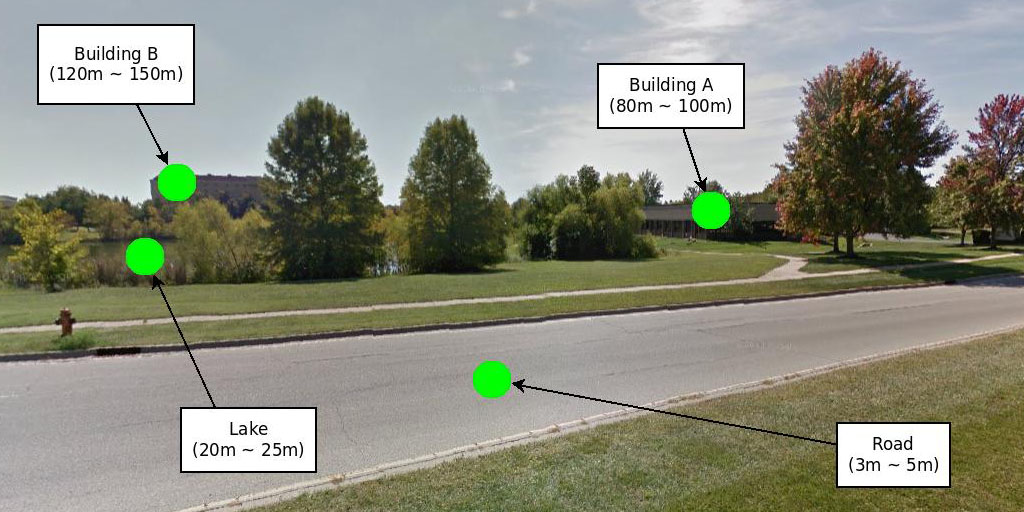
\includegraphics[width=.422\linewidth]{mcmc/streetview1}
    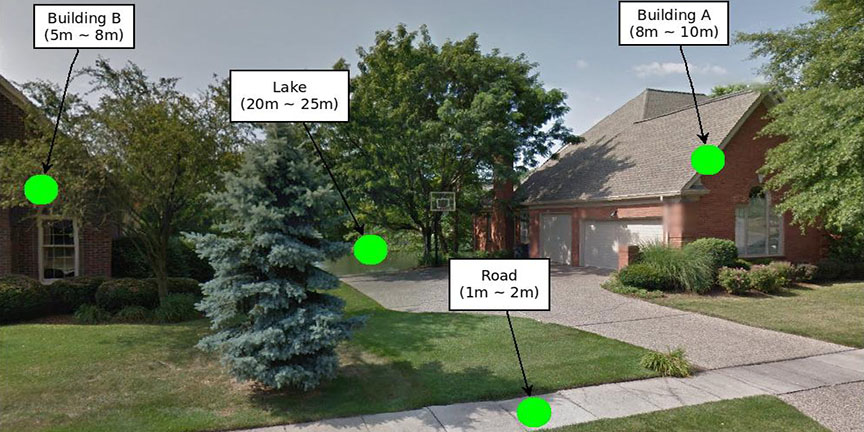
\includegraphics[width=.422\linewidth]{mcmc/streetview2}
    \caption{Query images}
  \end{subfigure}
  \begin{subfigure}{1\linewidth} 
    \centering
    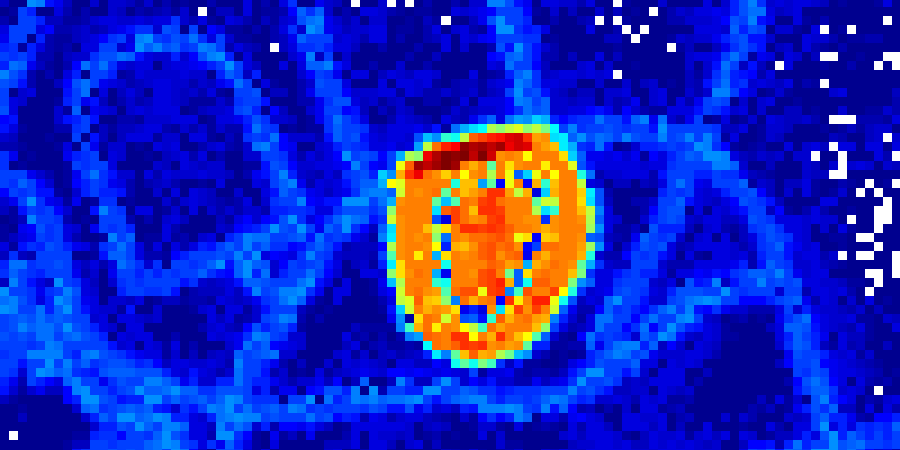
\includegraphics[width=.422\linewidth]{mcmc/streetview1_pdf}
    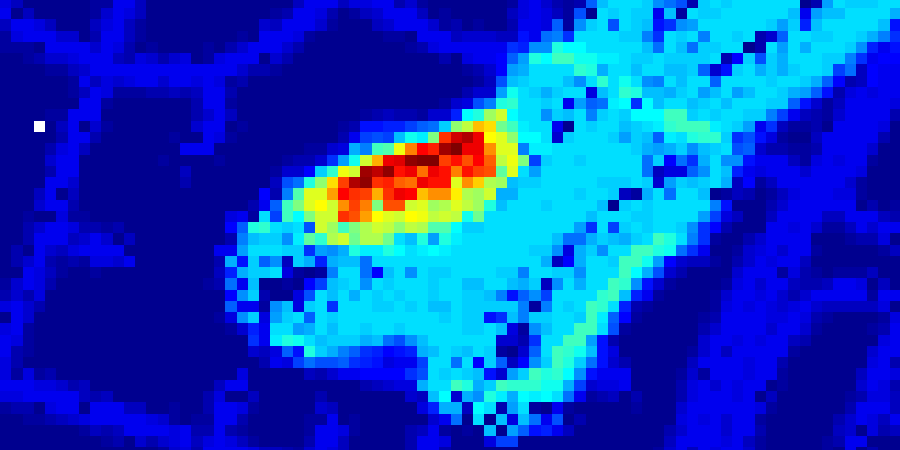
\includegraphics[width=.422\linewidth]{mcmc/streetview2_pdf}
    \caption{PDF of location}
  \end{subfigure}
  \begin{subfigure}{1\linewidth} 
    \centering
    \fbox{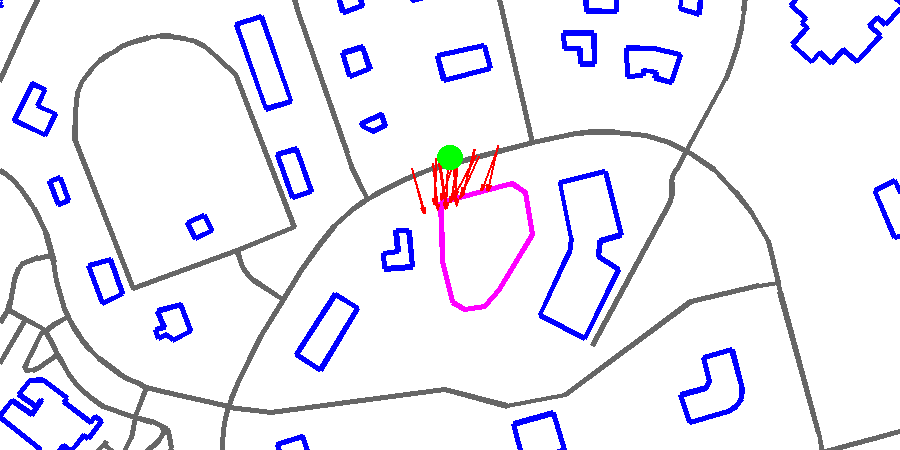
\includegraphics[width=.4\linewidth]{mcmc/streetview1_orient}}
    \fbox{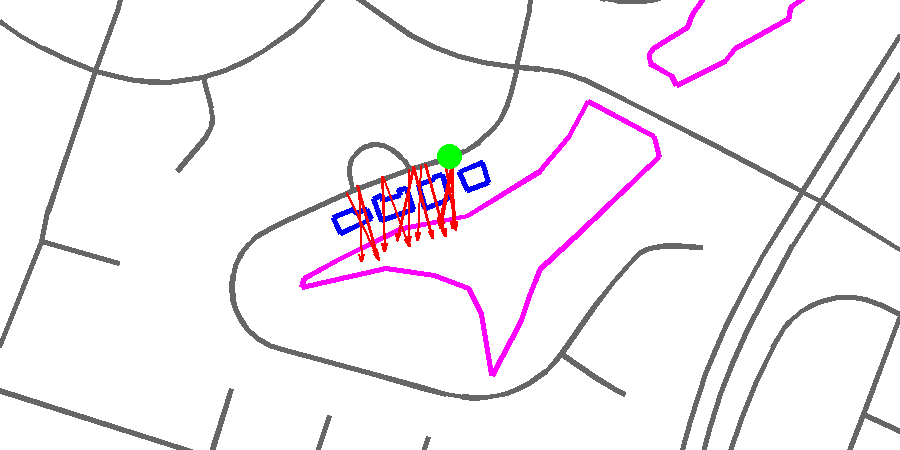
\includegraphics[width=.4\linewidth]{mcmc/streetview2_orient}}
    \caption{Local geographic database and top-15 samples}
  \end{subfigure}

  \caption{Qualitative results for two query images (top). The
  resulting PDFs (middle) and map visualization of the top-15 samples
(bottom) show that the proposed scoring function realistically
captures the  uncertainty.}

 \label{fig:real-data}
\end{figure}

We evaluate our method using two real query images obtained from
Google Street View. We hand-picked two locations, downloaded the
corresponding equirectangular panoramas and extracted a perspective
image from each. For each query, we labeled objects and estimated the
min/max distance from the camera to the object in the world.
\figref{real-data} shows the qualitative result of this experiment.
Our method generates high scoring samples that are close to the ground
truth. We also found that simple prior constraints can dramatically
affect localization accuracy. By restricting the range of the azimuth
and FOV to be within $5^\circ$ of the ground truth, the distance from
the top sample to the ground-truth location decreased from $12.5m$ to
$0.6m$ and from $1.73m$ to $0.9m$, respectively, for two test
cases.

%azimuth estimated from the sun position~\cite{lalonde2010sun}


\section{Conclusions}

We proposed an MCMC-based approach framework for single image camera
geo-calibration which leverages a large geographic database. Our
results demonstrate the superiority of our method versus several
baseline methods, without requiring nearby ground-level imagery as is
typical for most vision techniques.
While we applied only a small set of primitive constraints in this work,  
the proposed framework is able to take any kind of constraints.
In the following chapters, we will explore to develop more sophisticated
constraint functions.
